%Fragen an Lehmann
%Soll ich noch Literatur dazu ein binden?
%Welchen Controller könnte ich verwenden?

\chapter{Batterie}\label{introduction}
Eine essenzielle Komponente bei der Realisierung eines individuell konstruierten E-Bikes ist die Batterie, welche den Motor mit der benötigten Energie versorgt. Im vorliegenden Abschnitt wird detailliert auf die Fertigung einer individuellen Lithium-Ionen-Batterie eingegangen, die durch die Auswahl passenden Zellen und ihre spezifische Konfiguration realisiert wird.\\

%Was muss die Batterie Leisten?
Die Batterie muss den spezifizierten Anforderungen hinsichtlich Leistung, Form und Stabilität entsprechen. In Bezug auf die Leistung ist eine Spannung von 48 Volt erforderlich, um den Motor zu versorgen, und die Batterie muss eine Leistung von 1500 Watt bereitstellen, um die gewünschte Performance zu gewährleisten. Dies wird durch diese Formel berechnet\ref*{eq:wattformel}:\\
\begin{equation}
    P = U \cdot I \longrightarrow I = \frac{P}{U}= \frac{1500W}{48V}= 31.25
    \label{eq:wattformel}
\end{equation}
\label{introduction2}
%Welche Kapazität soll die Batterie haben?

Die Batterie sollte nicht nur die erforderliche Leistung liefern, sondern auch eine stabile und sichere Form aufweisen. Die physikalische Stabilität der Batterie ist entscheidend, um sicherzustellen, dass sie den Belastungen während des Betriebs standhält und keine strukturellen Schwächen aufweist.\\

Darüber hinaus ist die Form der Batterie relevant, da sie in das E-Bike integriert werden muss. Die Form sollte daher kompatibel mit dem vorgesehenen Platzierungsort sein, um eine effiziente Nutzung des verfügbaren Raums zu ermöglichen. Die Batterie sollte sich leicht und sicher im vorgesehenen Bereich befestigen lassen, um eine optimale Integration in das Gesamtsystem zu gewährleisten.\\

Die Konstruktion der Batterie stellt einen maßgeblichen Schritt im Bau eines selbstgefertigten E-Bikes dar, da sie maßgeblich die Leistung und Reichweite des Fahrzeugs beeinflusst.


\section{Zellen}
%Welche Rollen spielen die Zellen im Batterie bau?
Die Zellen in einer Lithium-Ionen-Batterie für E-Bikes spielen eine entscheidende Rolle bei der Speicherung und Bereitstellung elektrischer Energie. Jede Zelle fungiert als eigenständige Energieeinheit, die miteinander kombiniert werden, um die gewünschte Spannung und Kapazität für den E-Bike-Motor zu erreichen. Ihre Aufgaben umfassen die Speicherung von Elektronen während des Ladevorgangs und die Abgabe dieser Elektronen während des Entladevorgangs, um den Motor mit Strom zu versorgen.\\

%Wie werden sie verbunden?
Die Zellen werden in der Batterie durch spezifische Verbindungsmethoden miteinander verbunden. Die Verbindung erfolgt durch das serielle Schalten der Zellen, wodurch die Einzelspannungen addiert werden. Dieser Schritt ermöglicht es, die für den E-Bike-Motor erforderliche höhere Gesamtspannung von 48 Volt zu erreichen. Die meisten Zellen haben 3.6 Volt Nennspannung um auf die 48 Volt zu kommen müssen 13 in Reihe geschaltet werden.\\

%Wie ist der schaltplan?
Die Entscheidung, Zellen in Serie oder parallel zu schalten, beeinflusst maßgeblich die Leistung und Charakteristik der Batterie. Die Reihenschaltung erhöht die Gesamtspannung, während die Parallelschaltung die Gesamtkapazität steigert. Dies hat direkte Auswirkungen auf die Leistungsfähigkeit des E-Bikes. Eine geeignete Kombination von Reihen- und Parallelschaltungen kann die erforderliche Spannung und Kapazität optimieren und somit die Fahrleistung und Reichweite des E-Bikes verbessern.\\

nsgesamt spielen die Zellen im Lithium-Ionen-Batteriebau für E-Bikes eine zentrale Rolle, und ihre Verbindung durch Reihen- und Parallelschaltungen ist entscheidend für die Leistungsfähigkeit und Effizienz des Batteriesystems.\\


\subsection{Art der Zellen}
Bei der Art der Zellen kommen nur zwei in Frage einmal die 21700-Zellen und 18650-Zellen\ref*{fig:1850VS21700}.

\begin{figure}[h]
    \centering
    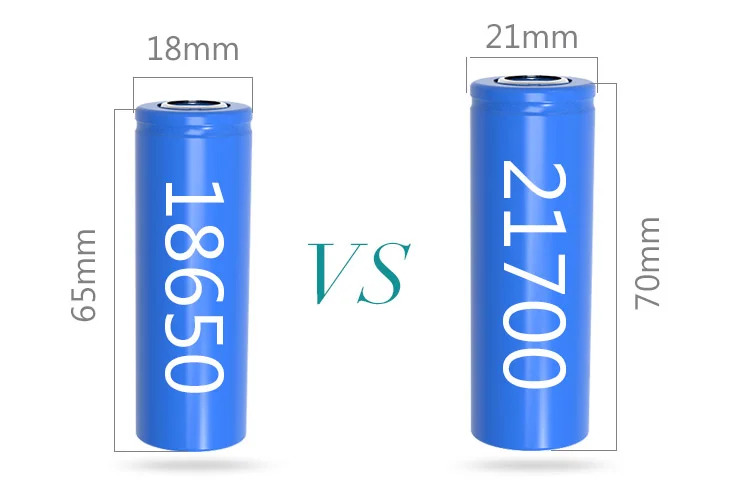
\includegraphics[width=8cm]{images/18650-VS-21700.jpg}
    \caption{1850 VS 21700\cite{Tritek.12132021}}
    \label{fig:1850VS21700}
\end{figure}

Die Entscheidung zwischen 21700-Zellen und 18650-Zellen für die Batteriekonstruktion von E-Bikes erfordert eine eingehende wissenschaftliche Analyse verschiedener Faktoren. Einer der entscheidenden Aspekte ist die energetische Leistung und Kapazität der Zellen. Die größeren Dimensionen der 21700-Zellen ermöglichen eine höhere Kapazität pro Zelle im Vergleich zu den kleineren 18650-Zellen, was zu einer potenziell höheren Energiedichte führt und somit die Gesamtkapazität und Reichweite der Batterie positiv beeinflussen kann.\\

21700-Zellen weisen oft niedrigere interne Widerstände im Vergleich zu 18650-Zellen auf. Dies bedeutet, dass weniger Energie in Form von Wärme verloren geht, während die Zellen betrieben werden. Ein niedrigerer interner Widerstand ermöglicht eine effizientere Nutzung der in der Batterie gespeicherten Energie und reduziert somit die Wärmeentwicklung während des Betriebs. Dies kann insgesamt zu einer besseren thermischen Leistungsfähigkeit der Batterie beitragen und potenzielle Überhitzungsprobleme verringern.\\

Die Verwendung von 21700-Zellen bietet eine Reihe von Vorteilen, die das Preis-Leistungs-Verhältnis im Vergleich zu 18650-Zellen verbessern. Zum einen sind 21700-Zellen aufgrund ihrer höheren Energiedichte kosteneffizienter, da sie eine größere Kapazität pro Zelle bieten. Dadurch wird weniger Zellen benötigt, um die gleiche Leistung zu erzielen, was zu Einsparungen sowohl bei den Material- als auch bei den Herstellungskosten führt. Zudem reduziert die Verwendung weniger Zellen das Risiko von Ausfällen und erfordert weniger Arbeitsaufwand für die Montage und Wartung.\\

%Darüber hinaus ermöglichen die technologischen Fortschritte, die mit der Einführung der 21700-Zellen einhergehen, die Integration neuerer Technologien. Diese könnten die Leistung, Sicherheit und Zuverlässigkeit der Batterien verbessern. Obwohl 18650-Zellen als etabliert und bewährt gelten, könnten die neueren 21700-Zellen von diesen Fortschritten in der Batterietechnologie profitieren.\\%kann auch weg gelassen werden

Zusammenfassend lässt die wissenschaftliche Analyse vermuten, dass die Verwendung von 21700-Zellen aufgrund ihrer potenziell höheren Kapazität, verbesserten Wärmeableitung und der Möglichkeit, von technologischen Fortschritten zu profitieren, für E-Bike-Batterien vorteilhaft sein könnte.

\subsection{Wahl der Marke}
Die beiden Zelltypen, Samsung und Lishen, unterscheiden sich in mehreren Schlüsselparametern, die bei der Entscheidung für die Batteriekonstruktion eines E-Bikes berücksichtigt werden sollten.\\

Die Samsung-Zellen zeichnen sich durch eine höhere Kapazität von 4900 mAh aus, was potenziell zu einer längeren Betriebsdauer des E-Bikes führen könnte. Allerdings liegt der maximale Entladestrom bei 9,8A pro Zelle, was die Leistungsfähigkeit des Motors beeinflussen kann. \\

Im Gegensatz dazu bietet die Lishen-Zelle eine Kapazität von 4000 mAh, was etwas niedriger ist als bei Samsung. Allerdings ermöglicht sie einen höheren maximalen Entladestrom von 12A pro Zelle. Ein zusätzlicher Vorteil könnte sein, dass die Lishen-Zellen preiswerter sind, was eine wirtschaftliche Alternative darstellen könnte.\\

In einer Batteriekonfiguration für E-Bikes spielt die Anzahl der parallel geschalteten Zellen eine entscheidende Rolle für die Entladeleistung. Wenn weniger Zellen parallel geschaltet sind, bedeutet dies, dass die Gesamtkapazität der Batterie reduziert ist. Um dennoch die erforderliche Leistung bereitzustellen, muss der Entladestrom pro Zelle erhöht werden. Es gibt auch Zellen die einen Entladestrom von 35 Amper liefern.

Die Entscheidung zwischen diesen Zellen hängt von den spezifischen Anforderungen des E-Bike-Projekts ab. Wenn eine längere Reichweite und eine höhere Kapazität priorisiert werden, könnten die Samsung-Zellen die bessere Wahl sein. Wenn jedoch eine höhere Leistungsfähigkeit des Motors und ein wirtschaftlicher Preis im Vordergrund stehen, könnte die Lishen-Zelle die geeignetere Option sein. Es ist ratsam, die Projektspezifikationen und das Budget sorgfältig zu prüfen, um die optimale Zellwahl zu treffen.\\

Es wurde sich für die Lishen-Zellen entschieden, da sie am billigsten waren und auch mehrer Parallel geschaltet werden um eine erhöhte Kapazität zuerreichen einher geht auch das genug Leistung von der Batterie geleistet werden kann. Es werden 13 Zellen in Reihe geschaltet um 48 Volt zuerreichen, 5 parallel für eine Kapazität von 20 Amperstunden und einen maximalen Entladestrom von 60 Amper. Hier ist die Berechnung: \ref*{eq:Strom}. Die Begründung warum genau fünf parallel geschaltet werden findet man hier:\ref{introduction}\\

\begin{align}
    A_{\textrm{Battery}} =& 12 A\cdot 5 = 60 A\\
    V_{\textrm{Battery}} =& 3.6V \cdot 13 = 46.8V\\
    \textrm{Kapazität} =& 4000mAh \cdot 5 = 20 Ah
    \label{eq:Strom}
\end{align}

Hier sieht ist der Schaltplan einer solchen Batterie mit BMS:\ref{fig:5}



%add schaltplan

\section{Battery Management Systems}
%Was ist ein BMS?asdfasdf
Ein entscheidender Aspekt bei der Konstruktion von Lithium-Ionen-Batterien für E-Bikes ist die Wahl des richtigen Battery Management Systems (BMS). Dieser Abschnitt erläutert die Funktionen, den Auswahlprozess und die Entscheidungsgrundlagen für die Verwendung eines Balancing-BMS anstelle eines BMS, das lediglich Überwachungsfunktionen bietet.\\
%Wie funkitoniert ein BMS?
Ein BMS ist ein elektronisches System, das die Leistung und Sicherheit von Lithium-Ionen-Batterien überwacht und regelt. In seiner Grundfunktion überwacht es Parameter wie Spannung, Strom, Temperatur und Ladezustand. Zudem bietet es Schutzmechanismen, um Überladung, Tiefentladung und Überhitzung zu verhindern.\\
%balanced VS only monetoring
Es gibt zwei Haupttypen von BMS: solche, die lediglich Überwachungsfunktionen bereitstellen, und solche, die auch ein sogenanntes Balancing implementieren. Balancing bedeutet, dass das BMS aktiv eingreift, um sicherzustellen, dass alle Zellen in der Batterie während des Lade- und Entladevorgangs ähnliche Spannungen aufweisen.\\

%Zweck und Vorteile eines Balancing-BMS:
Die Entscheidung für ein Balancing-BMS basiert auf der Notwendigkeit, eine gleichmäßige Verteilung der Spannung über alle Zellen hinweg sicherzustellen. Dieser Prozess ist entscheidend, um die Lebensdauer der Batterie zu verlängern und eine optimale Leistung zu gewährleisten. Im Gegensatz dazu konzentriert sich ein BMS mit ausschließlich Überwachungsfunktionen darauf, die Parameter zu überwachen, ohne aktiv in den Ladungsausgleich zwischen den Zellen einzugreifen.\\
%Warum ist es nicht gut wenn die Spannung der Zellen variert?
Die Variation der Spannung zwischen den Zellen in einer Batterie ist problematisch, da sie zu mehreren negativen Effekten führen kann, die die Leistungsfähigkeit, Sicherheit und Lebensdauer der Batterie beeinträchtigen.\\

Wenn die Spannung zwischen den Zellen variiert, kann dies zu einer ungleichmäßigen Entladung führen. Einige Zellen können schneller entladen werden als andere, was zu einem Ungleichgewicht in der Kapazitätsnutzung führt. Dies führt zu einer verkürzten Laufzeit und einer ineffizienten Nutzung der gesamten Batteriekapazität.\\

Eine Variation der Spannung birgt das Risiko von Überladung für einzelne Zellen. Wenn eine Zelle eine höhere Spannung aufweist als andere, besteht die Gefahr, dass sie über ihre Nennspannung hinausgeladen wird. Überladung kann zu einer thermischen Instabilität führen, was wiederum zu Sicherheitsrisiken wie Überhitzung, Bränden oder sogar Explosionen führen kann.\\

Umgekehrt kann eine zu niedrige Spannung in einer einzelnen Zelle bei Entladung auftreten. Dies kann zu einer Tiefentladung führen, was die Lebensdauer der Zelle drastisch verkürzt und zu irreparablen Schäden führen kann.\\

Ungleichmäßige Spannungsverteilung kann zu einer ungleichen Alterung der Zellen führen. Einige Zellen altern schneller als andere, was zu einem vorzeitigen Versagen der Batterie führen kann. Eine ausgeglichene Spannungsverteilung trägt dazu bei, die Lebensdauer der gesamten Batterie zu maximieren.\\

Eine ungleichmäßige Spannungsverteilung kann die Leistungsfähigkeit des Gesamtsystems beeinträchtigen. Insbesondere bei elektrischen Anwendungen wie E-Bikes kann dies zu einer unzureichenden Leistung und einer verringerten Reichweite führen.\\
%Begründung für die Entscheidung:
Die Wahl eines Balancing-BMS für die E-Bike-Batteriekonstruktion wurde aufgrund der Fokussierung auf eine maximal homogene Spannungsverteilung getroffen. Durch das aktive Balancing wird vermieden, dass einzelne Zellen aufgrund unterschiedlicher Lade- und Entladezyklen eine Ungleichgewichtssituation erfahren. Dies trägt nicht nur zur Verbesserung der Batterielebensdauer bei, sondern optimiert auch die gesamte Leistungsfähigkeit des E-Bike-Akkus.\\

Die Entscheidung für ein Balancing-BMS basierte auf der Zielsetzung, eine Batterie zu konstruieren, die nicht nur effizient und leistungsstark ist, sondern auch eine langfristige Zuverlässigkeit und Haltbarkeit gewährleistet. \ref{fig:5}\\
\begin{figure}[h]
    \centering
    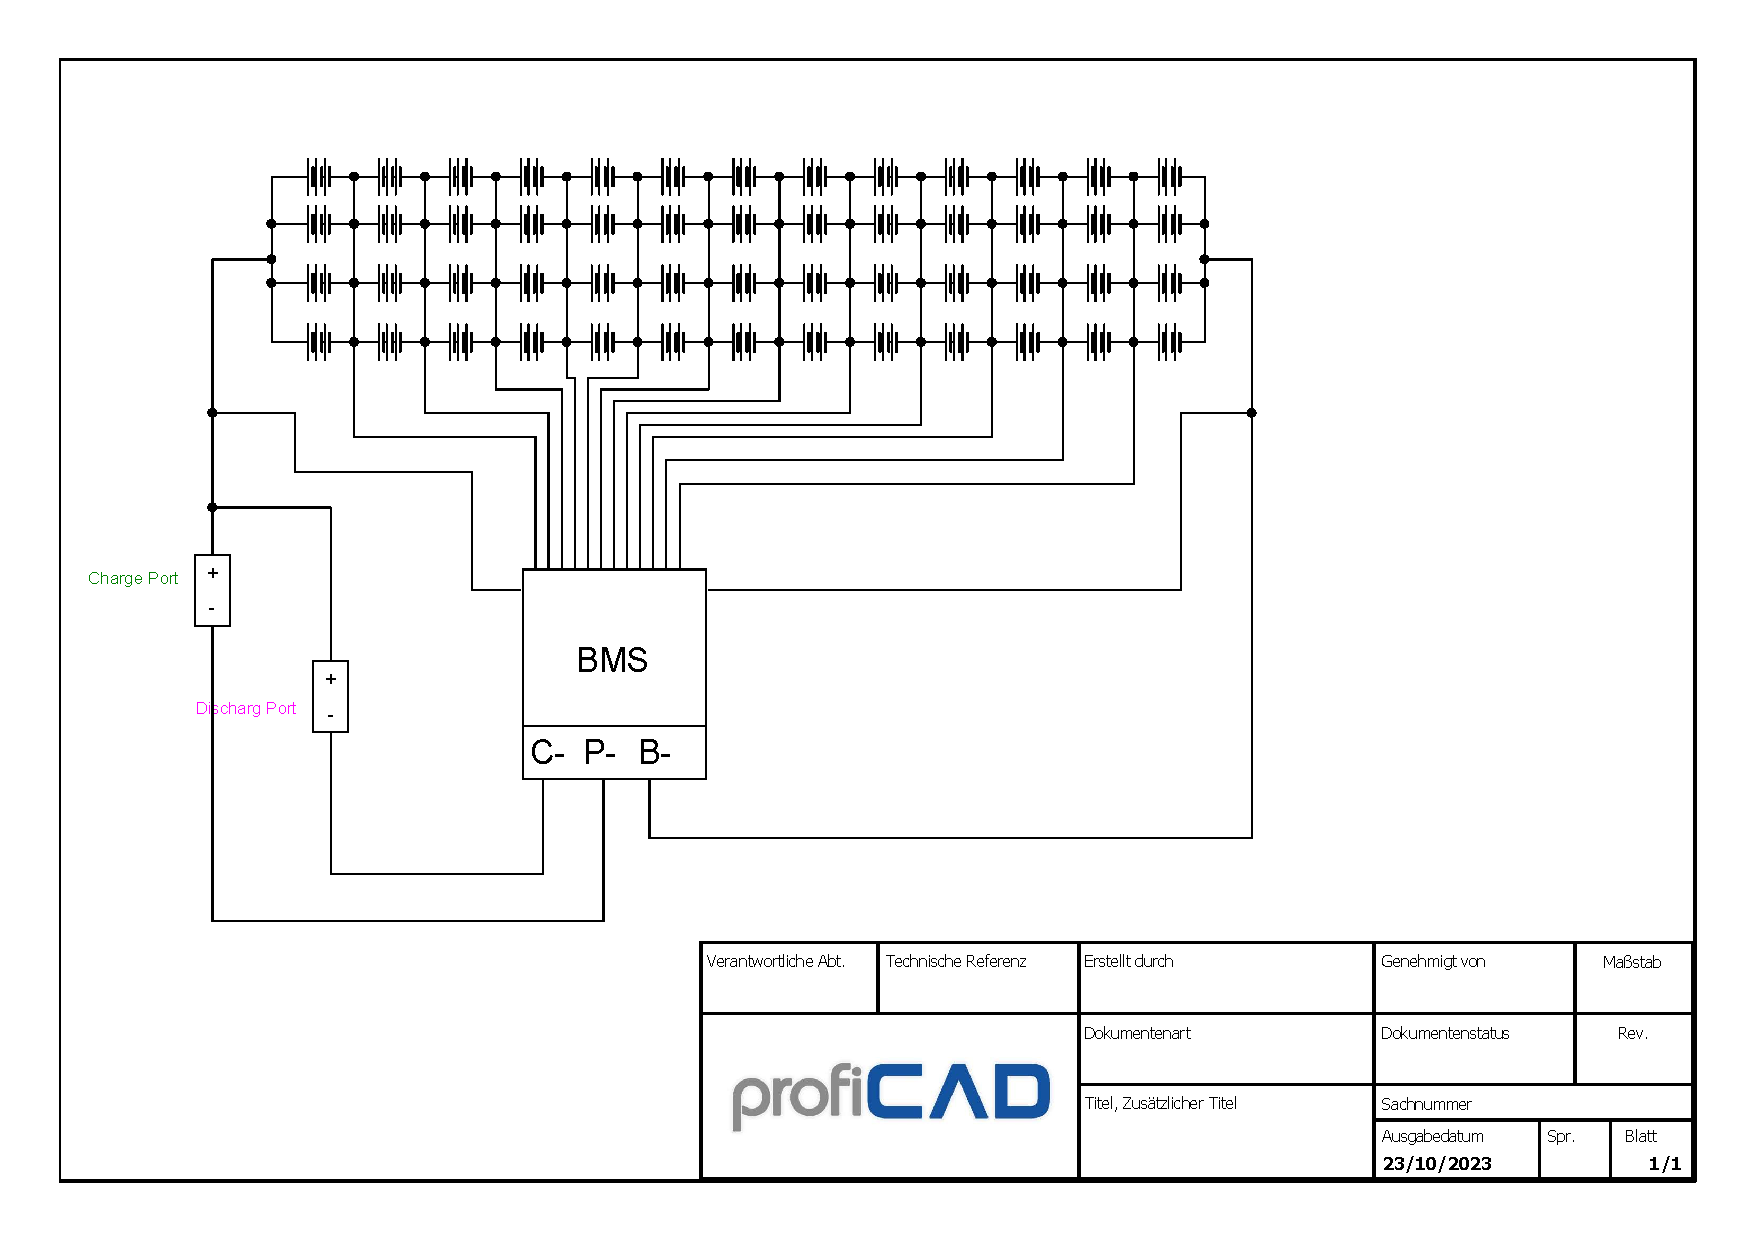
\includegraphics[width=10cm]{images/Schaltplan.pdf}
    \caption{Schaltplan\cite{LorenzScherrer.02.03.2024}}%
    \label{fig:5}
\end{figure}
Eine größere Version dieser Abbildung ist im Anhang zu finden.\ref{fig:5_1}
%Wozu braucht man ein BMS?

%Wovor schützt ein BMS?
%Für welches BMS wurde ich entschieden?

%Wie schließt man ein BMS an?
%Wie sieht der schaltplan aus?

\section{Verbindung zwischen den Zählen}

Die Verbindung zwischen den Zellen in einer Batterie kann auf verschiedene Weisen hergestellt werden, wobei die gängigsten Methoden das Punktzuschweißen, das Löten und das Verschrauben sind. Jede Methode hat ihre eigenen Vor- und Nachteile, und die Auswahl hängt von den spezifischen Anforderungen des Batteriedesigns ab.\\

Beim Punktzuschweißen werden dünnere Drähte oder Metallstreifen direkt an bestimmte Punkte auf den Batteriezellen geschweißt. Dies geschieht durch kurze elektrische Impulse, die einen Punkt auf der Zelle schmelzen und den Draht oder Streifen daran befestigen.\\

Beim Löten wird ein Lötzinn verwendet, um die Verbindungen zwischen den Zellen und den Verbindungselementen herzustellen. Dies kann mit einem Lötkolben erfolgen, der das Lötzinn schmilzt und es an Ort und Stelle hält, wenn es abkühlt.\\

Diese Methode beinhaltet das Anbringen von Metallfassungen an den Enden der Batteriezellen, die dann miteinander verschraubt werden. Die Fassungen dienen als Anschlusspunkte für die Verbindungselemente.\\

\subsection{Löten vs. Punktscheißen}
Die Wahl der geeigneten Methode zur Verbindung von Batteriezellen ist entscheidend für die Leistung, Sicherheit und Mobilität eines E-Bike-Batteriesystems. Angesichts der spezifischen Anforderungen und Einschränkungen wurde die Entscheidung getroffen, nur Löten und Punktschweißen in Betracht zu ziehen, wobei die Methode der mechanischen Verbindung mit Fassungen ausgeschlossen wurde.\\

%Beschränkungen der mechanischen Verbindung:
Die Methode der mechanischen Verbindung mit Fassungen wurde aus mehreren Gründen ausgeschlossen. Die schwere und kostspielige Natur dieser Methode erwies sich als unpraktisch für die Anzahl der Zellen in einer E-Bike-Batterie. Darüber hinaus war die mobile Verwendung des E-Bikes ein entscheidender Faktor, und eine zu komplexe mechanische Verbindung hätte die Tragbarkeit des Systems erheblich beeinträchtigt.\ref{fig:2}\\
%Bild von meschanischer Fassung
\begin{figure}[h]
    \centering
    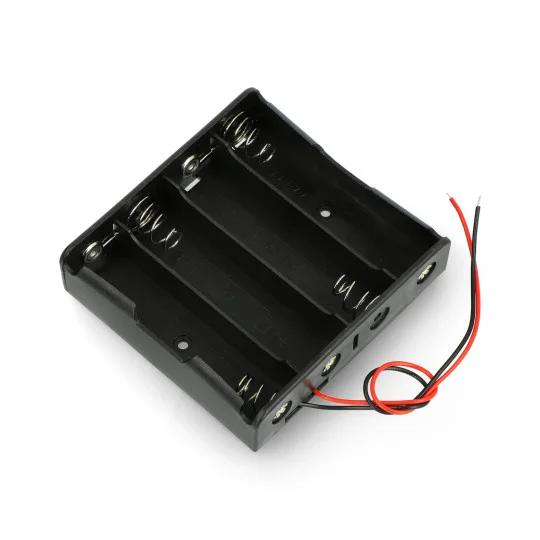
\includegraphics[width=8cm]{images/korb-fur-4-18650-akkus-reihenschaltung.png}
    \caption{Fassung für 18650 Batterie\cite{.02.03.2024}}%
    \label{fig:2}
\end{figure}


%Auswahl zwischen Löten und Punktschweißen:
Nach Ausschluss der mechanischen Verbindung blieben Löten und Punktschweißen als die beiden geeigneten Optionen für die Verbindung der Batteriezellen. Obwohl beide Methoden ihre Vor- und Nachteile haben, wurde eine fundierte Entscheidung getroffen, um den spezifischen Anforderungen gerecht zu werden.\ref{fig:3}\\
%Bild vom Punktschweißen
\begin{figure}[ht]
    \centering
    \includegraphics[width=8cm]{images/Punktschweißen_beispiel.jpg}
    \caption{Punktgeschweißte Verbindung\cite{LorenzScherrer.02.03.2024}}%\cite{selbst Experiment}
    \label{fig:3}
\end{figure}

%Löten als kosteneffiziente Option
Löten ist die kosteneffizientere Option mit dem geringern Beschaffungsaufwand, da es weniger spezielle Ausrüstung erfordert und leichter zugänglich ist. Die Einfachheit des Lötens ermöglichte eine effiziente Materialbeschaffung und eine schnellere Umsetzung. Obwohl Löten die Batterie durch die Wärmeentwicklung belasten kann und sie weniger Stabil ist. Diese Vermutung muss durch einen Test geprüft werden, da die andere Option nicht ohne weiters zugänglich ist.\ref{fig:4}\\
% Bild vom Löttest
\begin{figure}[ht]
    \centering
    \includegraphics[width=8cm]{images/Löten.png}
    \caption{Verbindung Löten\cite{LorenzScherrer.02.03.2024}}
    \label{fig:4}
\end{figure}

%Fazit
Das Punktgeschweißt werden der Batteriezellen wurde als bevorzugte Methode ausgewählt, da Löten aufgrund seiner Instabilität und des erhöhten Platzbedarfs mechanisch weniger praktikabel war. Die Auswahl der geeigneten Verbindungsmethode für Batteriezellen ist von entscheidender Bedeutung für Leistung, Sicherheit und Mobilität eines E-Bike-Batteriesystems. Angesichts der spezifischen Anforderungen und Einschränkungen erwies sich das Punktgeschweißt werden als die effizienteste Lösung, während die mechanische Verbindung mit Fassungen aus mehreren Gründen ausgeschlossen wurde. Die komplexe Natur und der hohe Platzbedarf der mechanischen Verbindung wären unpraktisch für die Anzahl der Zellen gewesen und hätten die Tragbarkeit des Systems beeinträchtigt. Nachdem die mechanische Verbindung ausgeschlossen war, blieben Löten und Punktschweißen als die beiden geeigneten Optionen für die Verbindung der Batteriezellen. Löten erwies sich als kosteneffizienter, erforderte jedoch einen Test, um die Stabilität zu bestätigen. Punktschweißen hingegen bot eine Standardlösung mit hoher Stabilität und geringerer Wärmeentwicklung auf den Batterien. Insgesamt wurde das Punktgeschweißt werden aufgrund seiner Effizienz und Zuverlässigkeit als bevorzugte Methode für die Verbindung der Batteriezellen für das E-Bike-Batteriesystem gewählt.\\



% Löten 
% -schnell
% -nicht stabil
% -es wurde ein test gemacht hier bild ein blenden
% -wenn nicht stabil hocher winderstand
% -Hitze auf den Batterien genau gefahren kann in die Luft gehen
% -Sicherung doch dünne drähte
% -mehr platz für 
% -Versuchsbeschreibung in einer Wissenschaftlichen Arbeit

% Punktzuschweißen
% -standard
% -sehr stabil
% -geringer Hitze auf den Batterien
% -

% Meschanisch verbinden
% -am besten und am sicherseten
% -kosten intensive
% -schwer viel platz wird gebraucht

\section{Punktschweißgerät}
%Wie funktioniert schweißen?

Das Punktschweißen ist ein gängiges Widerstandsschweißverfahren, das zur Verbindung von einem Blech und einer Zelle ohne den Einsatz von Zusatzwerkstoffen verwendet wird. Dabei werden die zu verbindenden Werkstücke durch die Erzeugung von Wärme an der Kontaktstelle verschmolzen und zu einer festen Verbindung vereint. Das Funktionsprinzip des Punktschweißens beruht auf der Nutzung elektrischen Stroms, um die erforderliche Wärmeenergie zu erzeugen und die Werkstücke zu verbinden.

\subsection{Funktionsweise des Punktschweißens}

%Bild vom Punktschweißen ein blenden

\begin{enumerate}
    \item \textbf{Ausrichtung der Werkstücke:} Zunächst werden die zu schweißenden Bleche präzise zueinander ausgerichtet, da eine nachträgliche Korrektur schwierig ist.
    \item \textbf{Anbringen und Aufpressen der Elektroden:} Zwei Elektroden, typischerweise aus Kupferlegierungen, werden auf die Oberflächen der Bleche aufgebracht und miteinander gepresst. Die Elektroden dienen dazu, den elektrischen Strom in die Schweißstelle zu leiten.
    \item \textbf{Erhitzung und Verflüssigung:} Durch den elektrischen Strom, der zwischen den Elektroden fließt, entsteht an der Kontaktstelle der Bleche Wärme. Diese führt dazu, dass das Material lokal schmilzt und die Bleche miteinander verschweißt werden.
    \item \textbf{Abkühlung und Erstarrung:} Nach Abschalten des Stroms erstarrt das geschmolzene Material und bildet eine feste Verbindung zwischen den Blechen. Der Druck der Elektroden wird während dieses Prozesses aufrechterhalten.
\end{enumerate}

\subsection{Erforderlicher Strom für das Punktschweißen}

Der für das Punktschweißen benötigte Strom hängt von verschiedenen Faktoren ab, darunter die Materialien der Werkstücke, ihre Dicke und die gewünschte Schweißqualität. Typischerweise liegt die erforderliche Stromstärke im Bereich von mehreren Hundert bis Tausend Ampere.

Die hohe Stromstärke ist notwendig, um ausreichend Wärmeenergie an der Schweißstelle zu erzeugen und die Bleche lokal aufzuschmelzen. Niedrigere Ströme würden nicht genügend Wärme erzeugen, um die erforderliche Schmelztemperatur zu erreichen.

Insgesamt ist das Punktschweißen ein effizientes Verfahren zur Herstellung von festen Verbindungen zwischen Blechen. Es erfordert einen geeigneten elektrischen Strom, um die erforderliche Wärmeenergie zu erzeugen und die Werkstücke erfolgreich zu verschweißen.

%Wie funktioniert ein Punktscheißgerät?


\subsection*{Transformator}
%Man braucht einen Transformator?

Ein Transformator wird beim Punktschweißen verwendet, um die erforderliche Stromstärke und Spannung für den Schweißprozess bereitzustellen.\\

%wie funktioniert einen transformator? %Wie funktioniert die Transformator formel?
Ein Transformator ist ein elektrisches Gerät, das verwendet wird, um die Spannung von Wechselstrom (AC) zu ändern. Es besteht aus zwei Spulen, die eng miteinander gekoppelt sind, aber elektrisch isoliert voneinander sind. Diese Spulen sind als Primär- und Sekundärwicklung bekannt.

%Abbildung von einen Transformator

Das Funktionsprinzip eines Transformators basiert auf elektromagnetischer Induktion. Wenn Wechselstrom durch die Primärwicklung fließt, erzeugt er ein wechselndes Magnetfeld um die Spule herum. Dieses Magnetfeld induziert eine Spannung in der Sekundärwicklung gemäß den Prinzipien der elektromagnetischen Induktion von Faraday.

%Wie muss man den transformator verändern? %Wie muss der Transformator gewickelt werden? 

Die Verhältnisse der Windungen in der Primär- und Sekundärwicklung bestimmen die resultierende Spannungsumwandlung. Wenn die Anzahl der Windungen in der Sekundärwicklung größer ist als die in der Primärwicklung, wird die Spannung im Verhältnis erhöht (Step-Up-Transformator). Wenn die Anzahl der Windungen in der Sekundärwicklung kleiner ist als die in der Primärwicklung, wird die Spannung im Verhältnis reduziert (Step-Down-Transformator).

%Wo bekommt man einen transformator her?


Ein Mirkowelen-Transformator eingnet sich sehr gut für den bau eines Punktschweißgerät.


Um herauszufinden, wie der sekundäre Block gewickelrt werden muss, kann die Transformatorformel verwendet werden.\ref{eq:3}

Transformator Formel:
\begin{align}%
        \frac{U_s}{U_p} &= \frac{N_s}{N_p}\\
        \frac{U_s}{U_p}\cdot N_p &= N_s \\
        \frac{I_s}{I_p} &=\frac{N_p}{N_s}\\
        \frac{I_p}{I_s} \cdot N_p = N_s &= \frac{16A}{800A}\cdot 224 \approx 4.48
        \label{eq:3}
\end{align}
        
        \begin{conditions*}
            U_p  &  Spannung am primären Block\\
            U_s  &  Spannung am sekundären Block $\approx 4V$ \\
            I_p  &  Stromstärke am primären Block = 16A\\
            I_s & Stromstärke am sekundären Block\\
            N_p & Wicklungen primären Block = $16\cdot14=224$\\
            N_s & Wicklungen sekundären Block\\
        \end{conditions*}



%Wie kann man den Sekundären Block sicher entfernen?
Jetzt muss der sekundäre Block entfernt werden um hin neu zu wickeln. \ref{eq:3}

Der Block muss auf einer Seite mit einer Stahlsäge durchtrennt werden und dann heraus geschalagen werden.

%Bilder vom entfernen des Blocks

%Weitere Probleme?

%Versuchs beschreibung in einer Wissenschaftlichen arbeit?
%Neuer Transformator?





%Wie schaltet man das Punktschweißgerät ein?
%Controller
%schalter
%Taster

\section{Konstruktion der Batterie}

Es wurde beschlossen, die Zellen mit doppelseitigem Klebeband anstatt mit Heißkleber zu verbinden.

%Bilder von der Batterie

Anschließend wurden alle Zellen punktverschweißt, sowohl in Reihe als auch parallel geschaltet. Die Anschlüsse des Batteriemanagementsystems (BMS) wurden gemäß dem Blockschaltbild \ref{fig:5_1} an die jeweilige Zellreihe angeschlossen. Nach Abschluss dieser Schritte wurde das Batteriepack mit einer Umwicklung aus Katonasch und Kaptonband isoliert. Diese Maßnahme diente dazu, die Zellen vor äußeren Einflüssen zu schützen und potenzielle Kurzschlüsse zu vermeiden. Nach der Isolierung konnte das Batteriepack erfolgreich mit einem Ladegerät geladen werden.


